\documentclass[12pt]{article}

% ---------- Page & Fonts ----------
\usepackage[a4paper, margin=2.5cm]{geometry}
\usepackage{xeCJK}
\usepackage{fontspec}
\setCJKmainfont{Songti SC} % macOS 常见字体；若报错可改为 SimSun/Source Han Serif SC

% ---------- Figures / Tables ----------
\usepackage{graphicx}
\usepackage{float}
\usepackage{booktabs}
\usepackage{caption}
\usepackage{subcaption}
\usepackage{hyperref}
\usepackage{indentfirst}
\setlength{\parindent}{2em}

\hypersetup{
  colorlinks=true,
  linkcolor=blue,
  urlcolor=blue,
  citecolor=blue
}

\title{2025年12月—2026年1月\\资金面、银行负债与利率曲线跟踪报告}
\author{Eli Ren}
\date{\today}

\begin{document}
\maketitle

\section*{摘要}

2025年12月至2026年1月期间，资金面在跨年阶段出现明显波动，
DR007阶段性冲高，但隔夜资金利率相对稳定，
显示流动性压力主要集中在期限结构层面。
公开市场操作在利率冲高阶段加大净投放规模，
短期资金面迅速修复，整体未形成趋势性收紧。

银行负债端方面，同业存单利率在回购利率冲高阶段保持相对平稳，
NCD-DR007利差短暂收窄后迅速修复，
表明短端流动性冲击未向中期负债端持续传导。

收益率曲线在12月末阶段性走陡，
进入1月后逐步回归平缓，
长端收益率与短端资金利率出现一定分化。
宏观层面，1月社融规模显著扩张，
MLF净投放同步放量，
但PMI重新回落至荣枯线以下，
CPI与PPI仍处低位区间，
信用扩张向实体景气的传导仍需进一步观察。

总体来看，本阶段市场特征表现为
“短期流动性扰动 + 政策对冲修复 + 信用阶段性放量 + 实体景气尚未同步改善”，
利率运行环境仍以震荡为主。

\clearpage
\renewcommand{\contentsname}{目录}
\tableofcontents
\clearpage

% =========================
\section{资金面：DR001 / DR007 与 OMO 对冲}
% =========================

\subsection{DR001 vs DR007：期限结构性紧张的识别}
\begin{figure}[H]
\centering
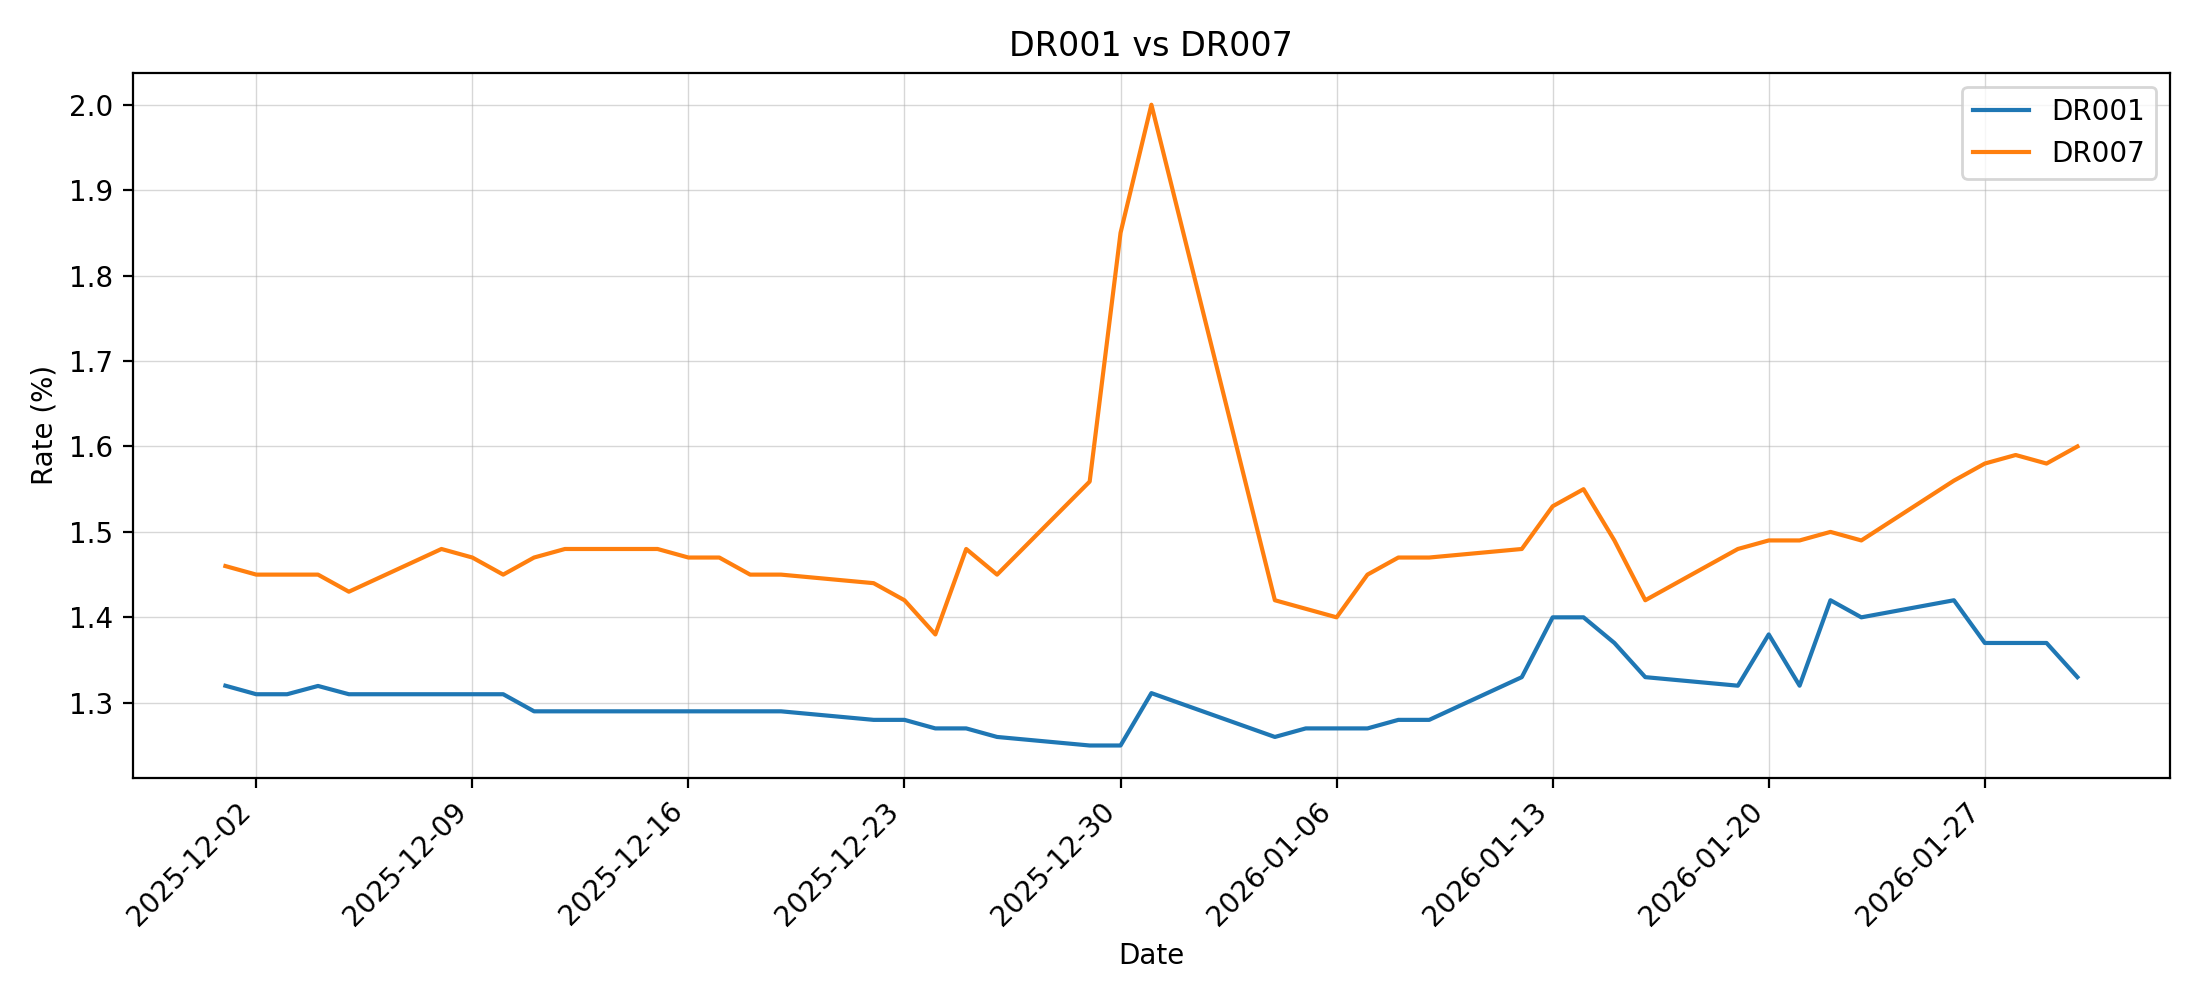
\includegraphics[width=0.92\textwidth]{figures/dr001_dr007.png}
\caption{DR001 vs DR007}
\end{figure}

2025年12月初至12月下旬，DR001维持在1.30\%附近小幅波动，
DR007在1.45\%左右运行，二者利差整体稳定。
12月末，DR007快速上行并一度接近2.0\%，
而DR001仅小幅抬升至1.31\%附近，
7天利率上行幅度显著高于隔夜利率。
这一现象表明跨年阶段的资金紧张主要集中在7天期限，
呈现明显的期限结构性特征，
而非全面流动性收紧。
进入2026年1月后，DR007迅速回落至1.40\%附近，
随后缓慢回升至1.60\%区间，
显示资金面由跨年冲击后的宽松状态
逐步回归至相对中性水平。

\subsection{DR007 vs OMO 7D净投放：政策对冲与利率回落}
\begin{figure}[H]
\centering
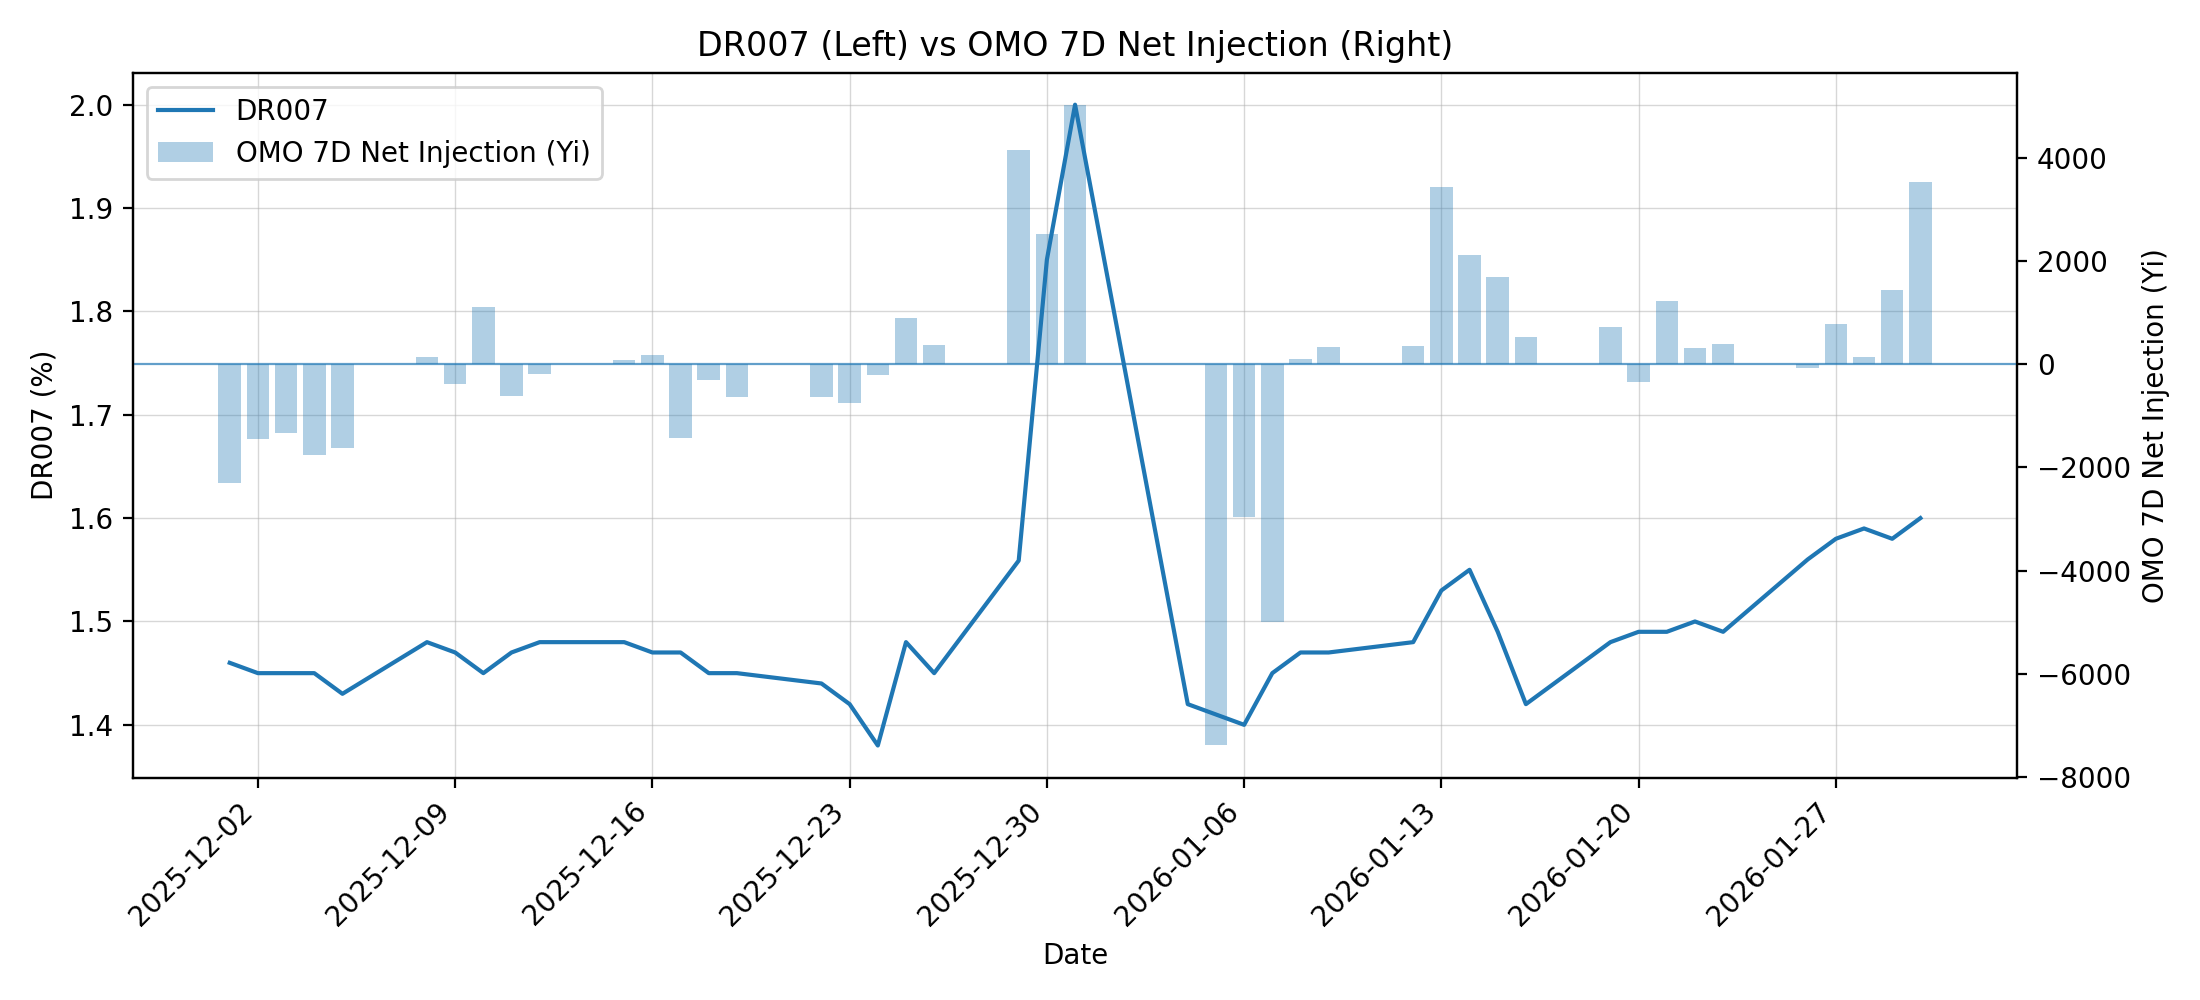
\includegraphics[width=0.92\textwidth]{figures/dr007_vs_omo_net.png}
\caption{DR007（左轴）与 OMO 7D 净投放（右轴）}
\end{figure}

在12月末DR007快速上行期间，
公开市场操作净投放规模显著增加，
单日净投放规模超过4000亿元。
随着投放放量，
DR007在数日内快速回落至1.40\%附近。
这一过程显示公开市场操作对短期流动性波动具有明显对冲作用，
本轮利率冲高更多属于短期资金错配，
并未体现政策方向性的收紧。
1月中旬以后净投放规模有所回落，
DR007中枢小幅抬升，
资金面整体进入平稳区间。

% =========================
\section{银行负债：NCD水平与利差（流动性/压力指标）}
% =========================

\subsection{NCD AAA（3M/6M/1Y）与 DR007：短端冲击是否传导到中期负债}
\begin{figure}[H]
\centering
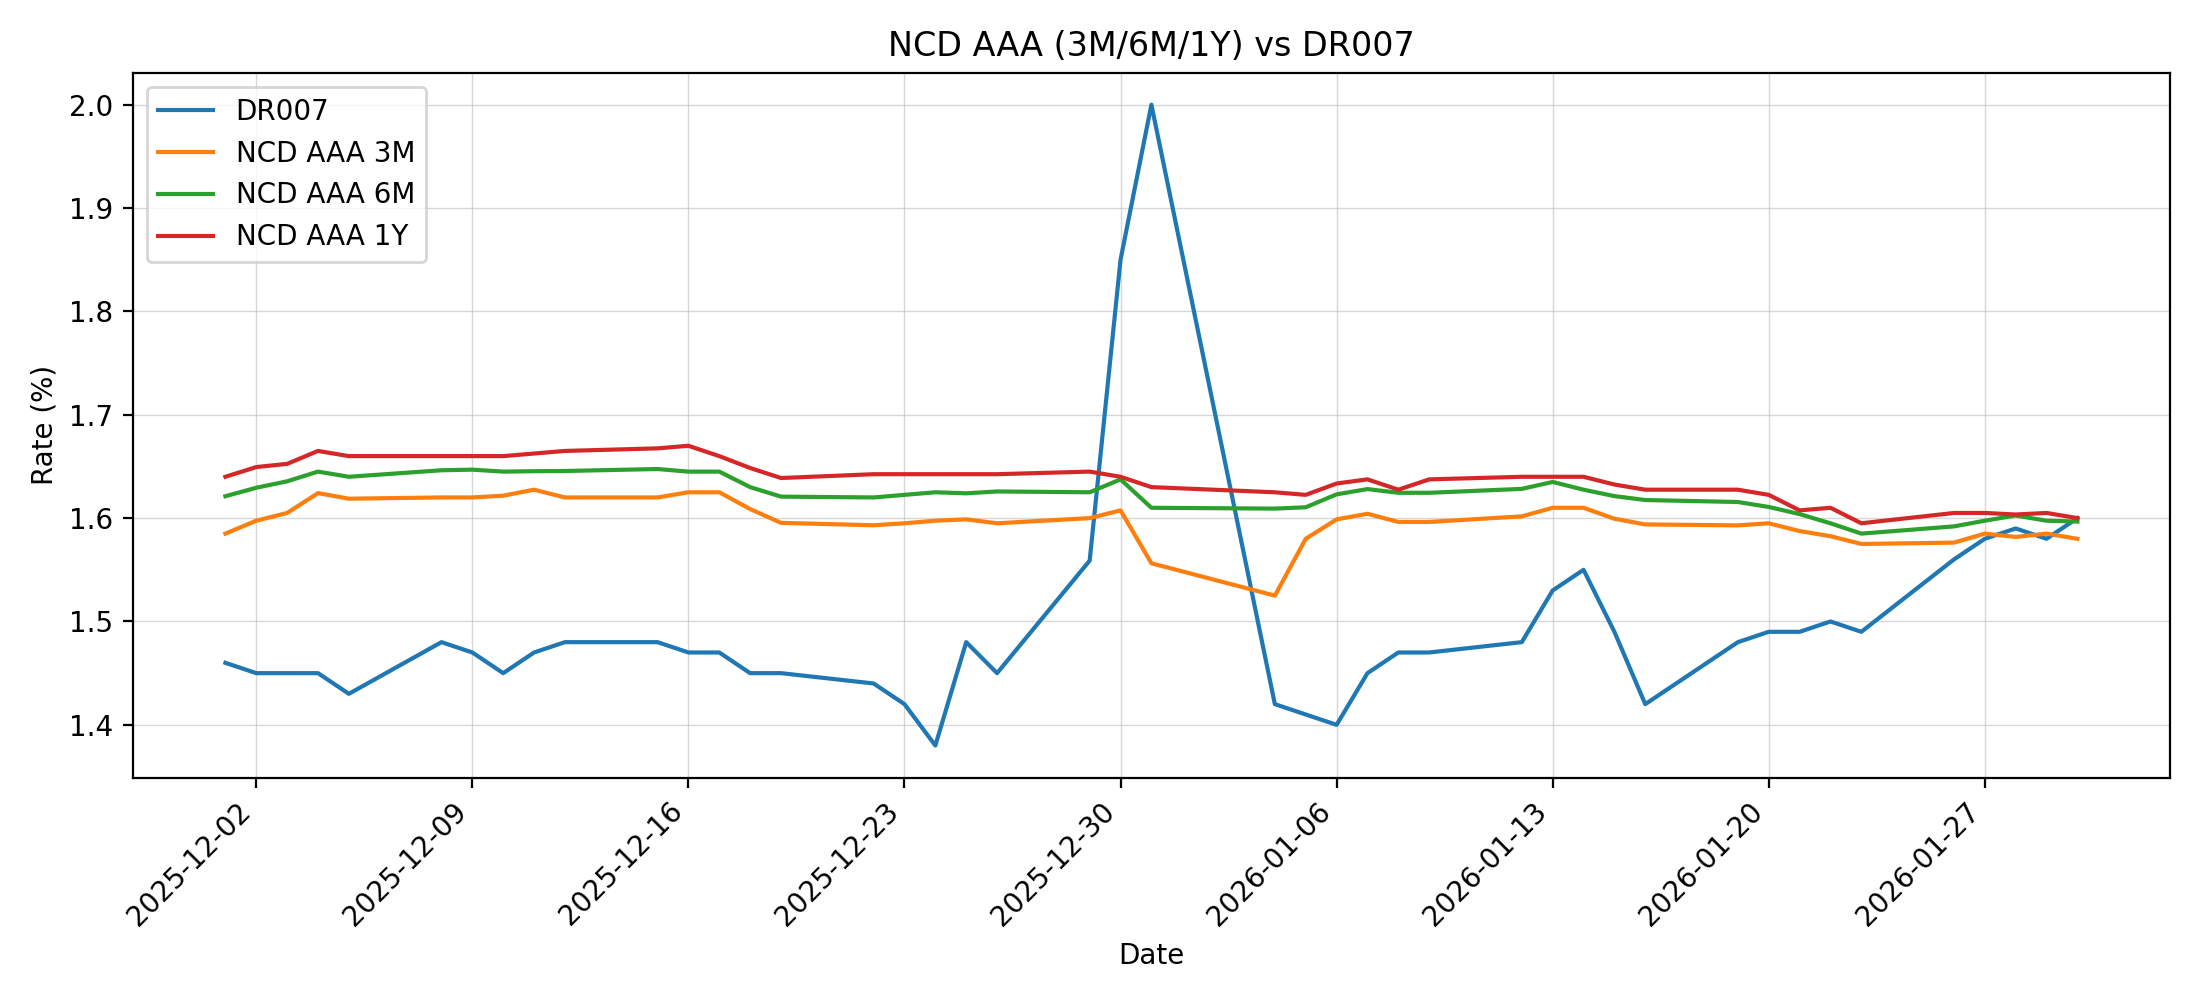
\includegraphics[width=0.92\textwidth]{figures/ncd_vs_dr007.png}
\caption{NCD AAA（3M/6M/1Y） vs DR007}
\end{figure}

12月大部分时间内，
NCD 3M、6M、1Y利率维持在1.58\%-1.65\%区间，
波动较为平稳。
在12月末DR007冲高至2.0\%期间，
NCD利率并未出现同步大幅上行，
整体保持稳定。
这一表现说明短端回购利率的冲击
未向银行中期负债成本持续传导，
市场对流动性紧张的持续性预期有限。
进入1月后，
随着DR007回落，
NCD利率小幅下行，
期限结构保持稳定。

\subsection{NCD利差：NCD-DR007 的压力刻画}
\begin{figure}[H]
\centering
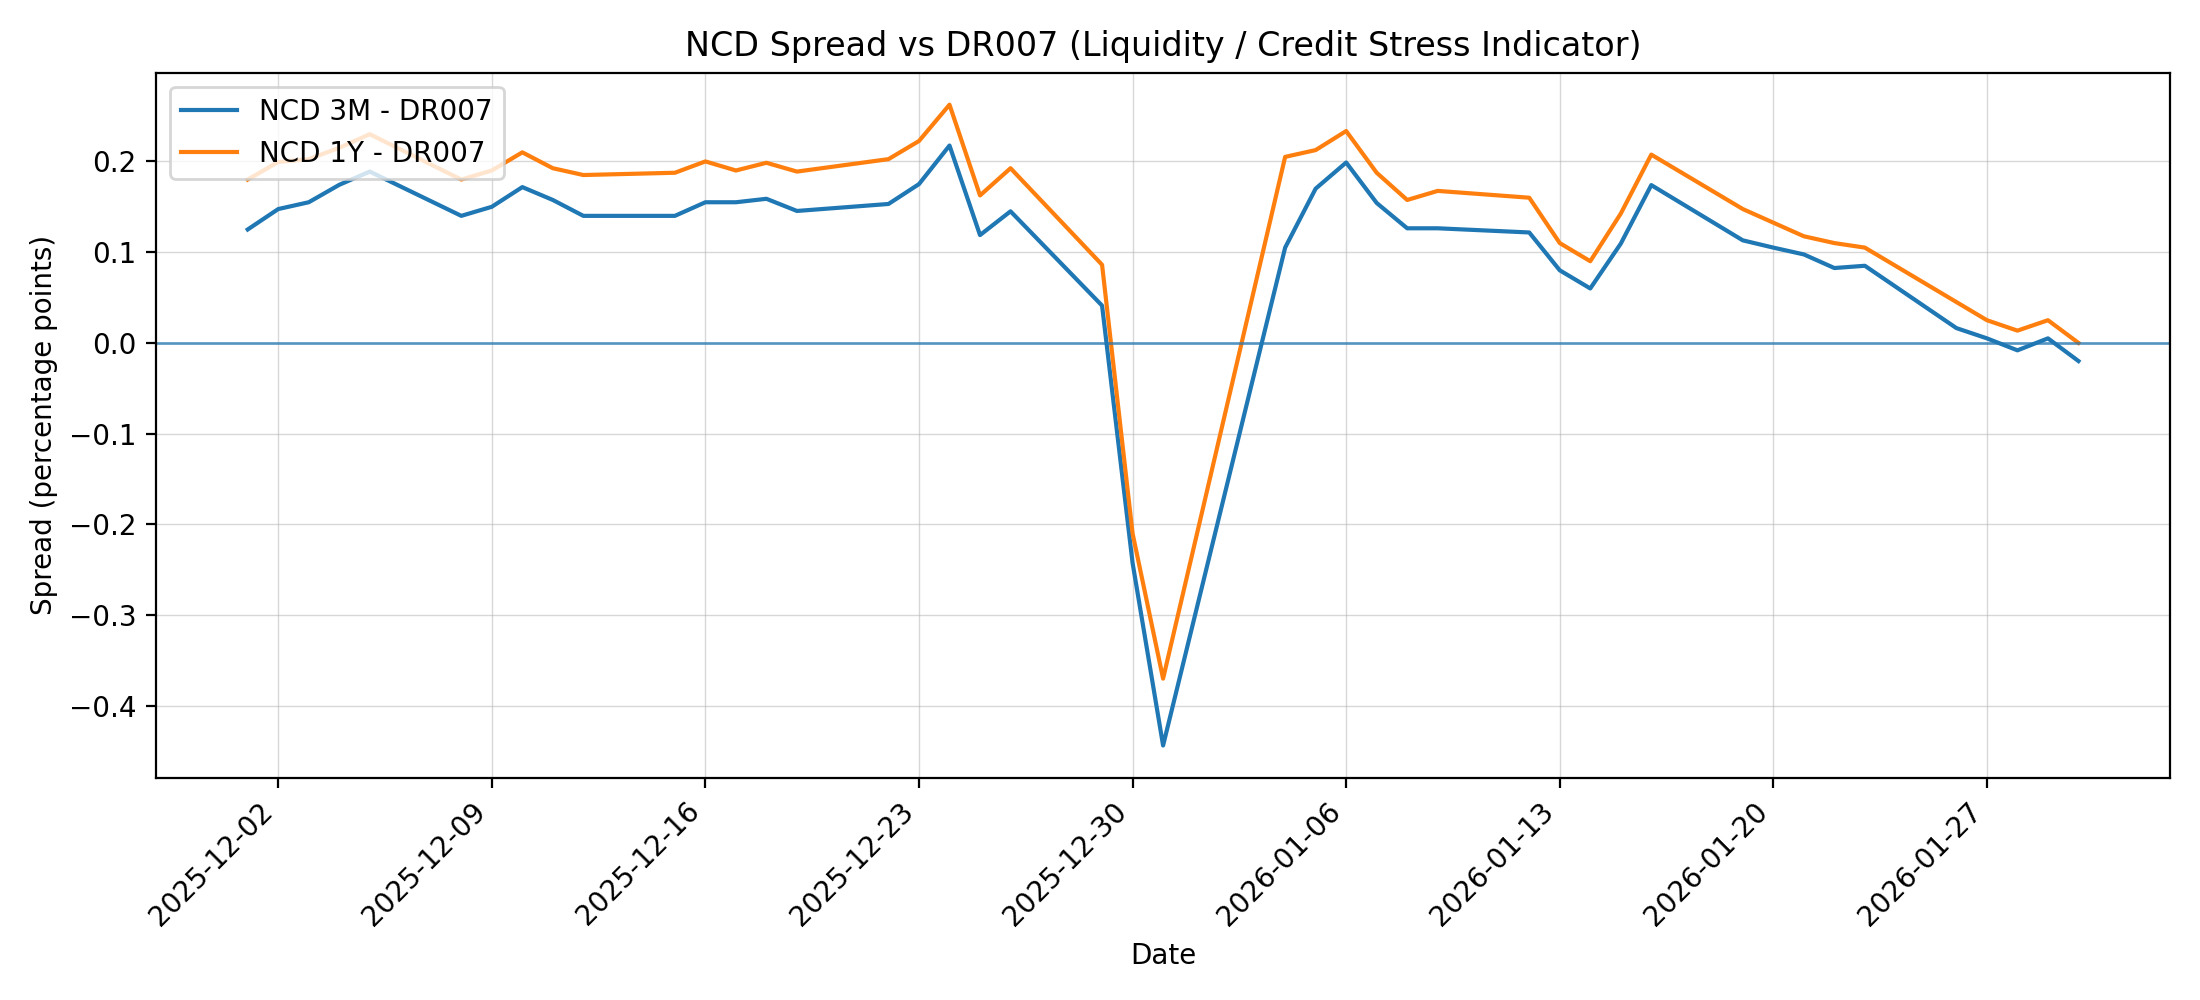
\includegraphics[width=0.92\textwidth]{figures/ncd_spread_vs_dr007.png}
\caption{NCD Spread vs DR007（Liquidity/Credit Stress Indicator）}
\end{figure}

12月初至12月下旬，
NCD 3M - DR007与NCD 1Y - DR007维持在0.15-0.20个百分点的正值区间。
12月末随着DR007快速上行，
利差显著收窄并短暂转负，
最低接近-0.40个百分点。
利差转负表明回购融资成本阶段性高于存单发行成本，
资金压力集中于短端。
进入1月初，
随着DR007回落，
利差迅速恢复至正值区间，
显示银行负债端未形成持续性紧张。

% =========================
\section{利率曲线：期限利差、曲线形态与长端定价}
% =========================

\subsection{期限利差：10Y-1Y 与 10Y-3M}
\begin{figure}[H]
\centering
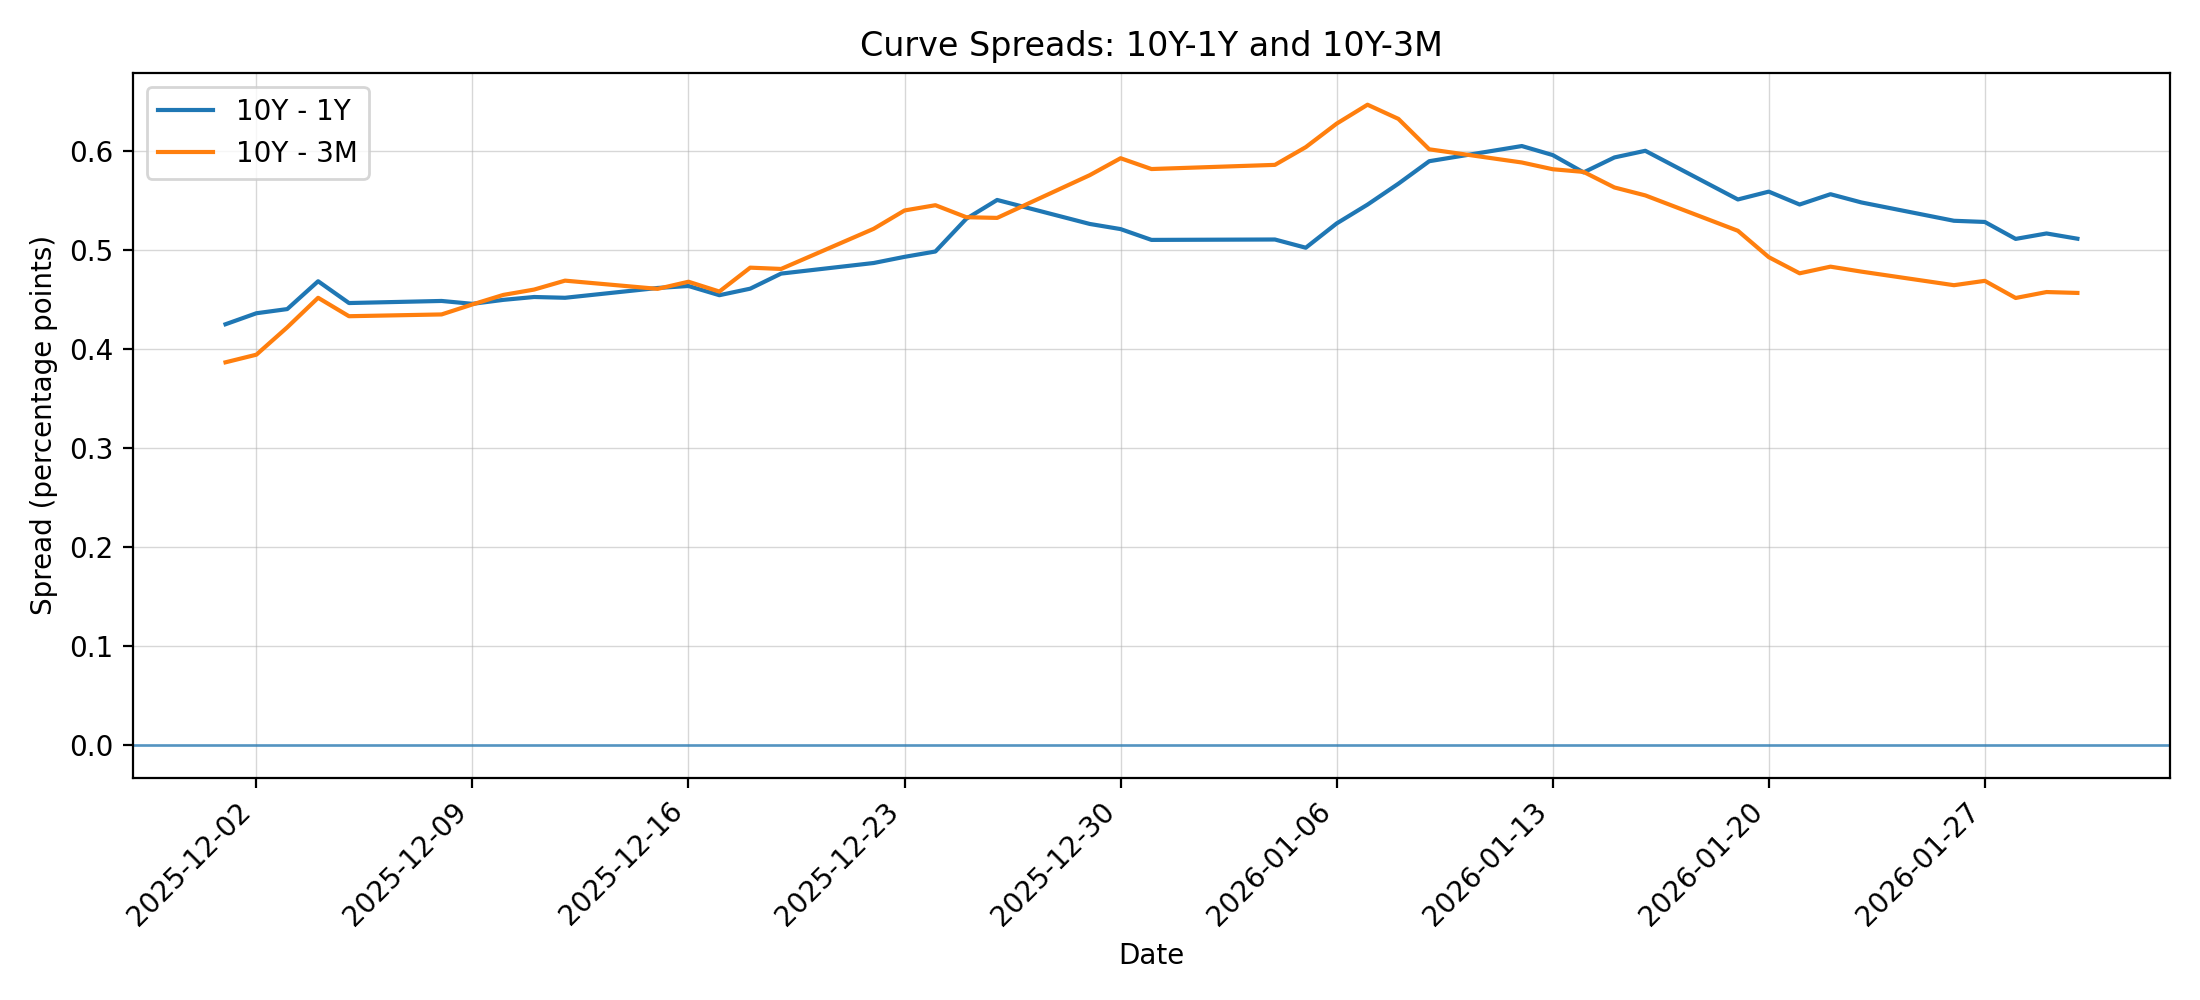
\includegraphics[width=0.92\textwidth]{figures/curve_spreads_10y_1y_10y_3m.png}
\caption{Curve Spreads: 10Y-1Y and 10Y-3M}
\end{figure}

12月期间，
10Y-1Y与10Y-3M利差整体缓慢扩大，
由约0.40个百分点上行至0.60个百分点附近。
这一阶段曲线走陡，
主要源于短端利率阶段性抬升。
进入1月中旬后，
利差逐步回落，
曲线重新趋于平缓。
曲线形态的变化
更多体现短端资金扰动的阶段性影响，
而非长端收益率趋势性调整。

\subsection{收益率曲线快照：2025-12-01 vs 2026-01-30}
\begin{figure}[H]
\centering
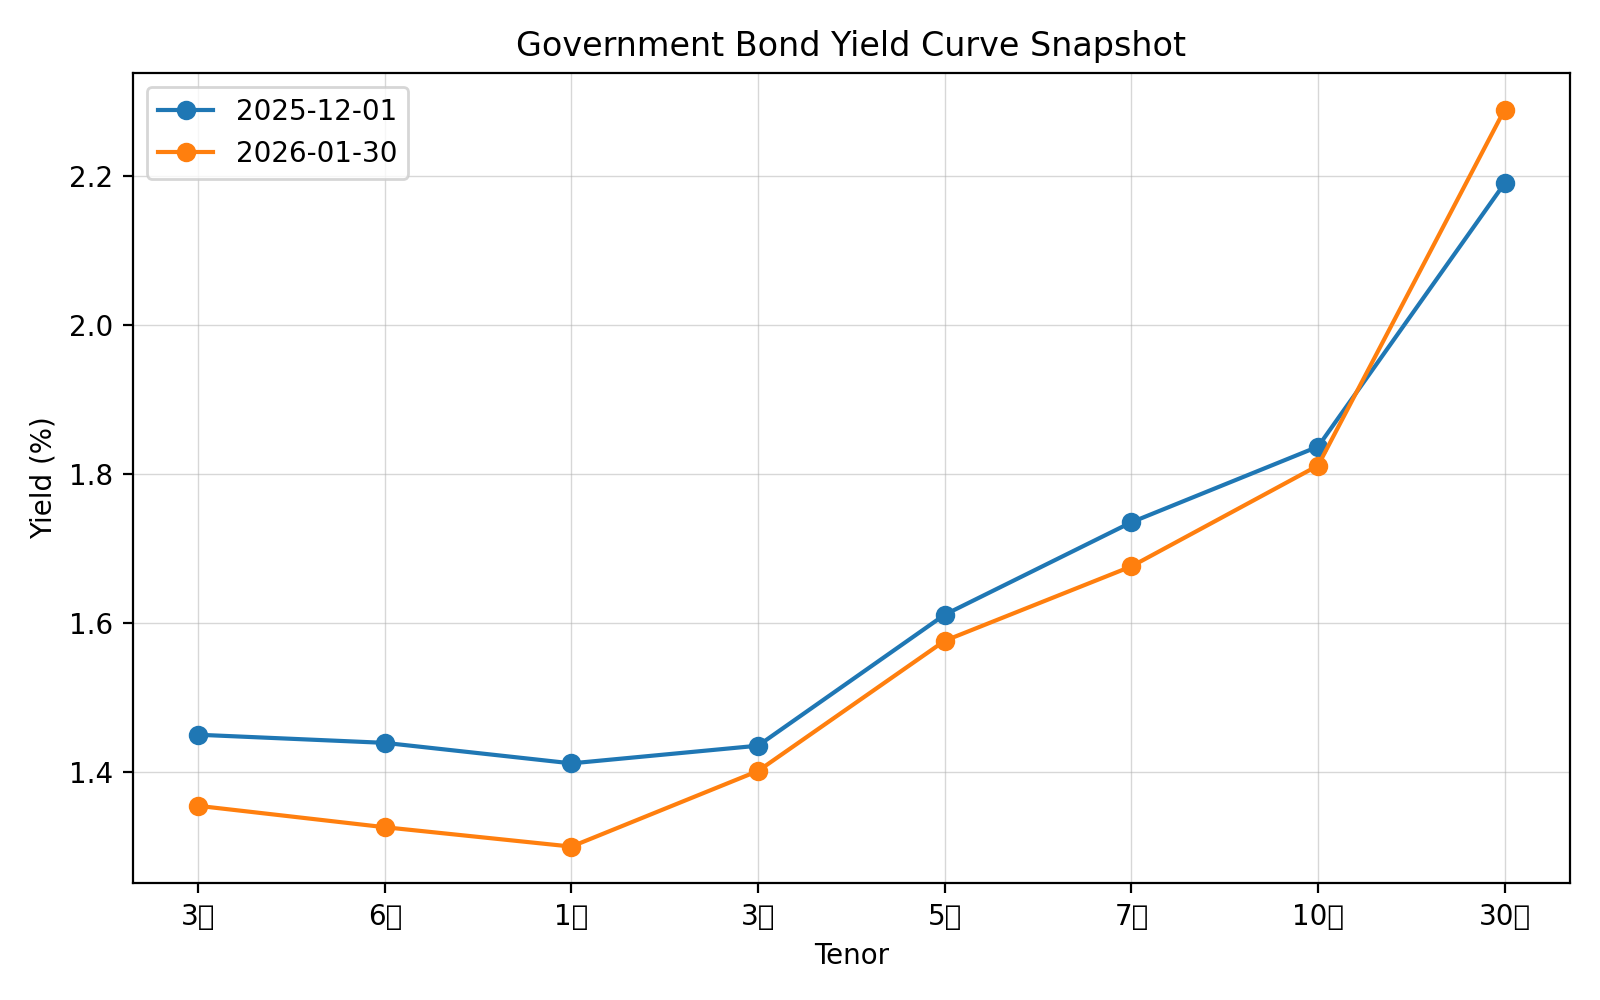
\includegraphics[width=0.92\textwidth]{figures/yield_curve_snapshot.png}
\caption{Government Bond Yield Curve Snapshot}
\end{figure}

2025年12月1日，
收益率曲线呈现平缓上行结构，
3M约1.45\%，
1Y约1.41\%，
10Y约1.84\%，
30Y约2.19\%。
2026年1月30日，
短端收益率整体下移，
3M降至1.35\%，
1Y降至1.30\%附近；
同时30Y收益率小幅上行至2.28\%。
曲线呈现短端回落、超长端抬升的结构，
反映流动性改善与长端定价因素并存。

\subsection{10Y vs DR007：资金面与长端的“脱钩/再耦合”}
\begin{figure}[H]
\centering
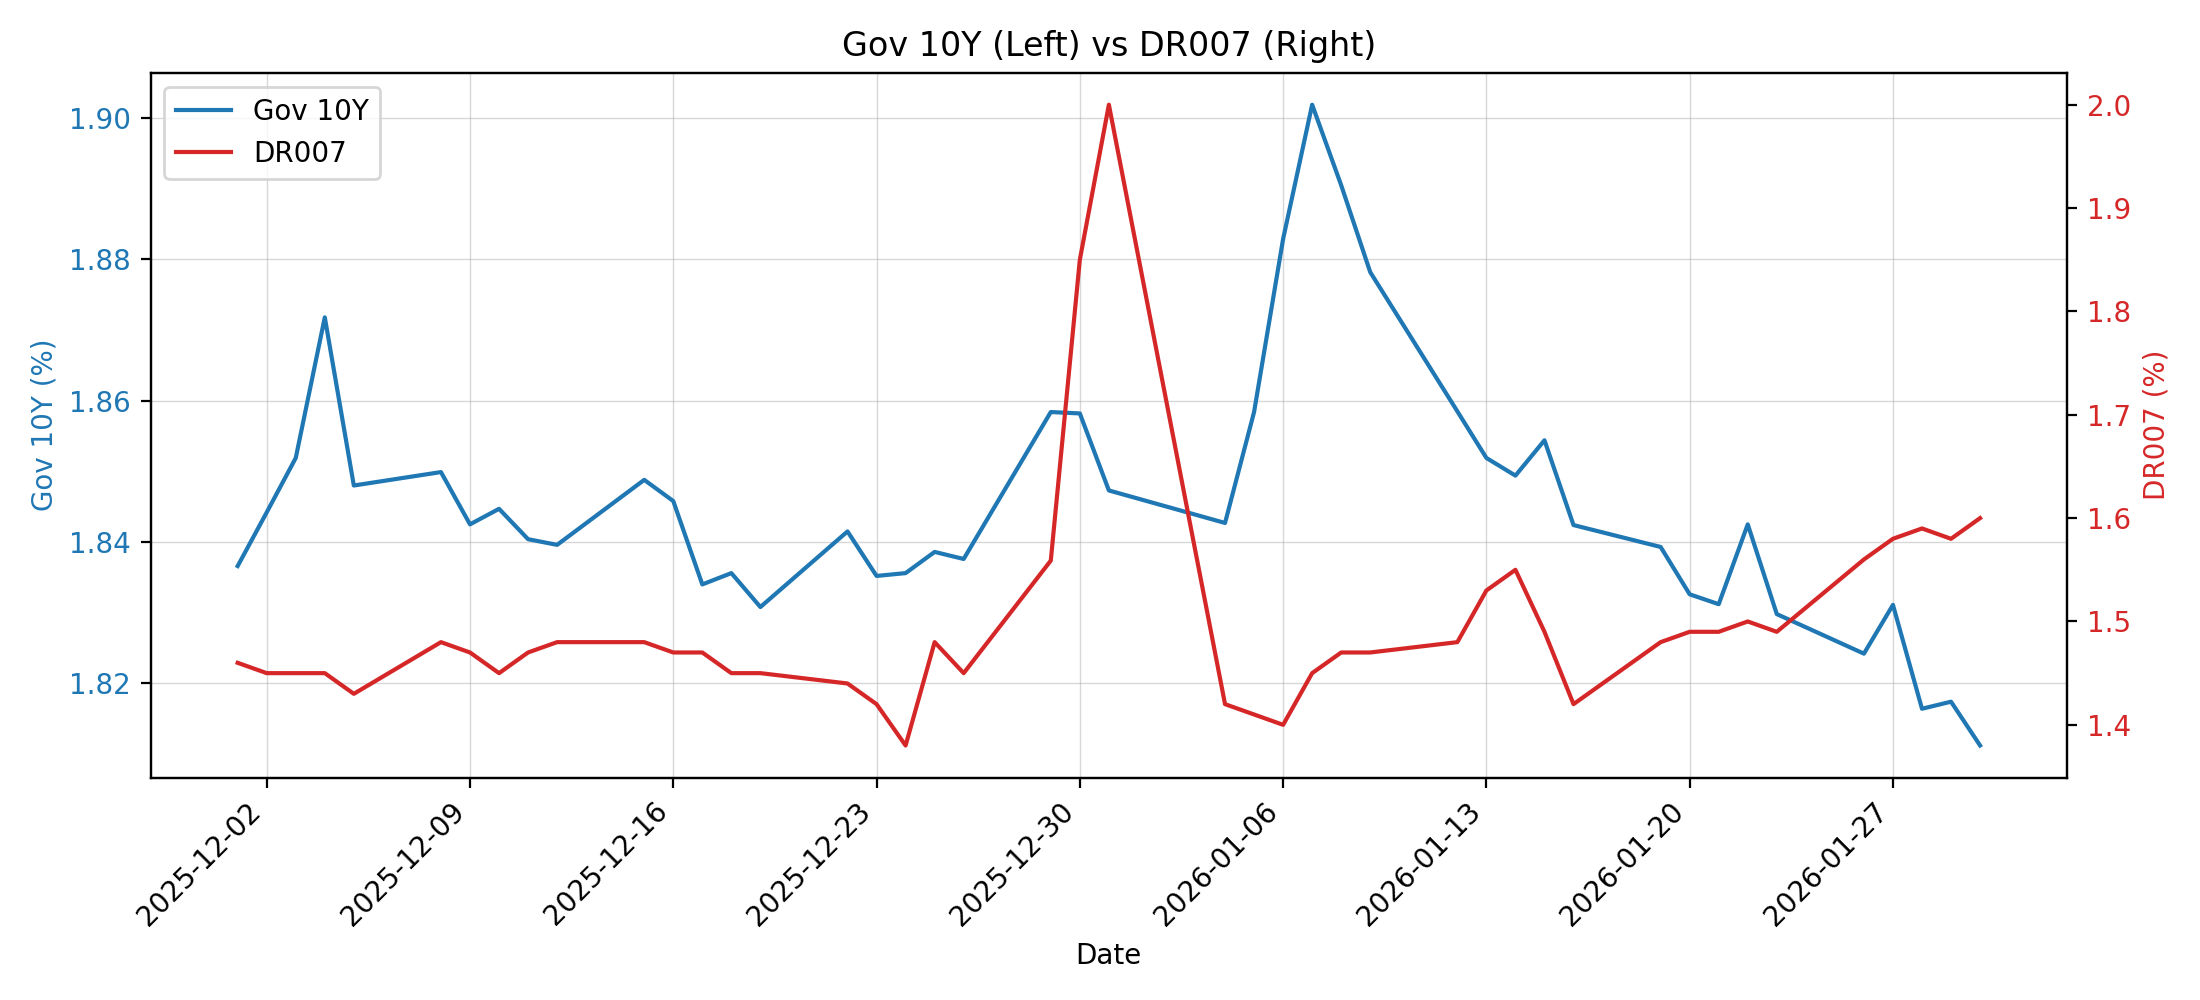
\includegraphics[width=0.92\textwidth]{figures/10y_vs_dr007.png}
\caption{Gov 10Y（左轴） vs DR007（右轴）}
\end{figure}

12月末DR007冲高阶段，
10Y国债收益率整体维持在1.85\%附近，
未出现同步显著上行，
显示长端未将短期资金冲击视为趋势信号。
1月上旬DR007回落后，
10Y收益率一度上行至1.90\%上方，
随后在1月下旬回落至1.82\%附近。
两者走势阶段性分化，
说明长端收益率的变化
并非完全由短端流动性驱动。

% =========================
\section{宏观：社融结构、PMI与通胀（CPI/PPI）}
% =========================

\subsection{社融结构拆分：贷款、票据与债券}
\begin{figure}[H]
\centering
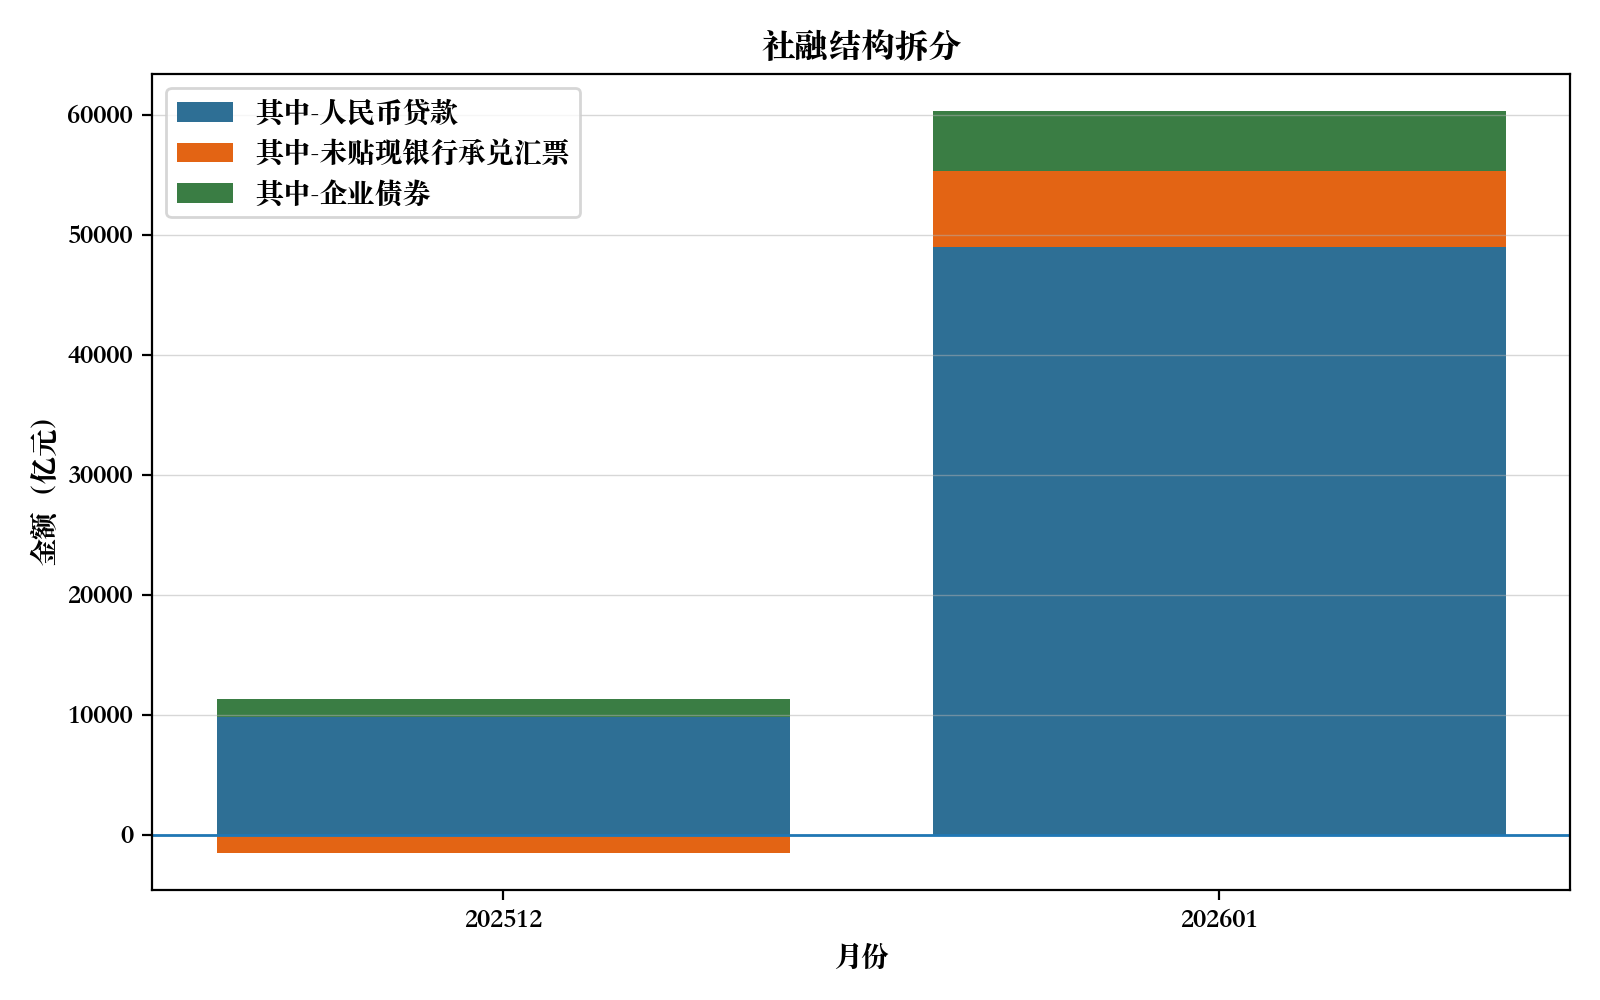
\includegraphics[width=0.92\textwidth]{figures/social_structure_stacked.png}
\caption{社融结构拆分}
\end{figure}

2025年12月，
人民币贷款约1万亿元，
未贴现银行承兑汇票为负值，
企业债券规模较小。
2026年1月，
人民币贷款上升至近5万亿元，
票据转为正值，
企业债券规模亦有所增加，
社融规模整体显著扩张。
社融放量显示信用供给阶段性增强，
但结构变化仍需结合实体景气数据观察其可持续性。

\subsection{PMI：景气线附近的边际变化}
\begin{figure}[H]
\centering
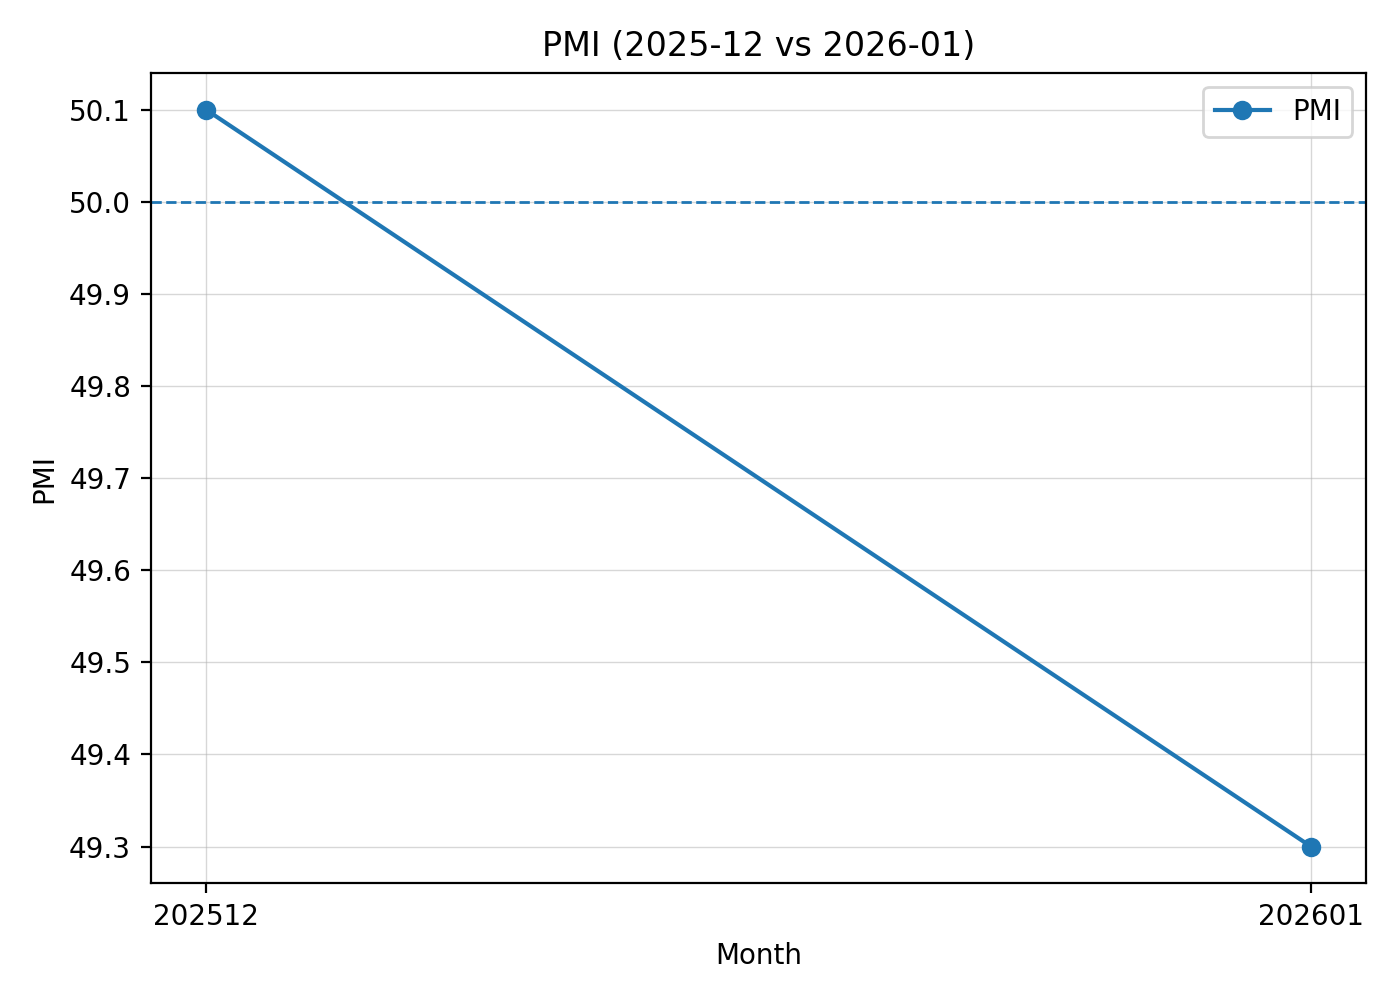
\includegraphics[width=0.80\textwidth]{figures/pmi_last2.png}
\caption{PMI（2025-12 vs 2026-01）}
\end{figure}

2025年12月PMI为50.1，
略高于荣枯线；
2026年1月回落至49.3，
重新进入收缩区间。
景气指标回落表明实体需求改善仍不稳固，
信用扩张与生产景气尚未形成同步改善。

\subsection{CPI \& PPI：通胀/通缩环境对长端的约束}
\begin{figure}[H]
\centering
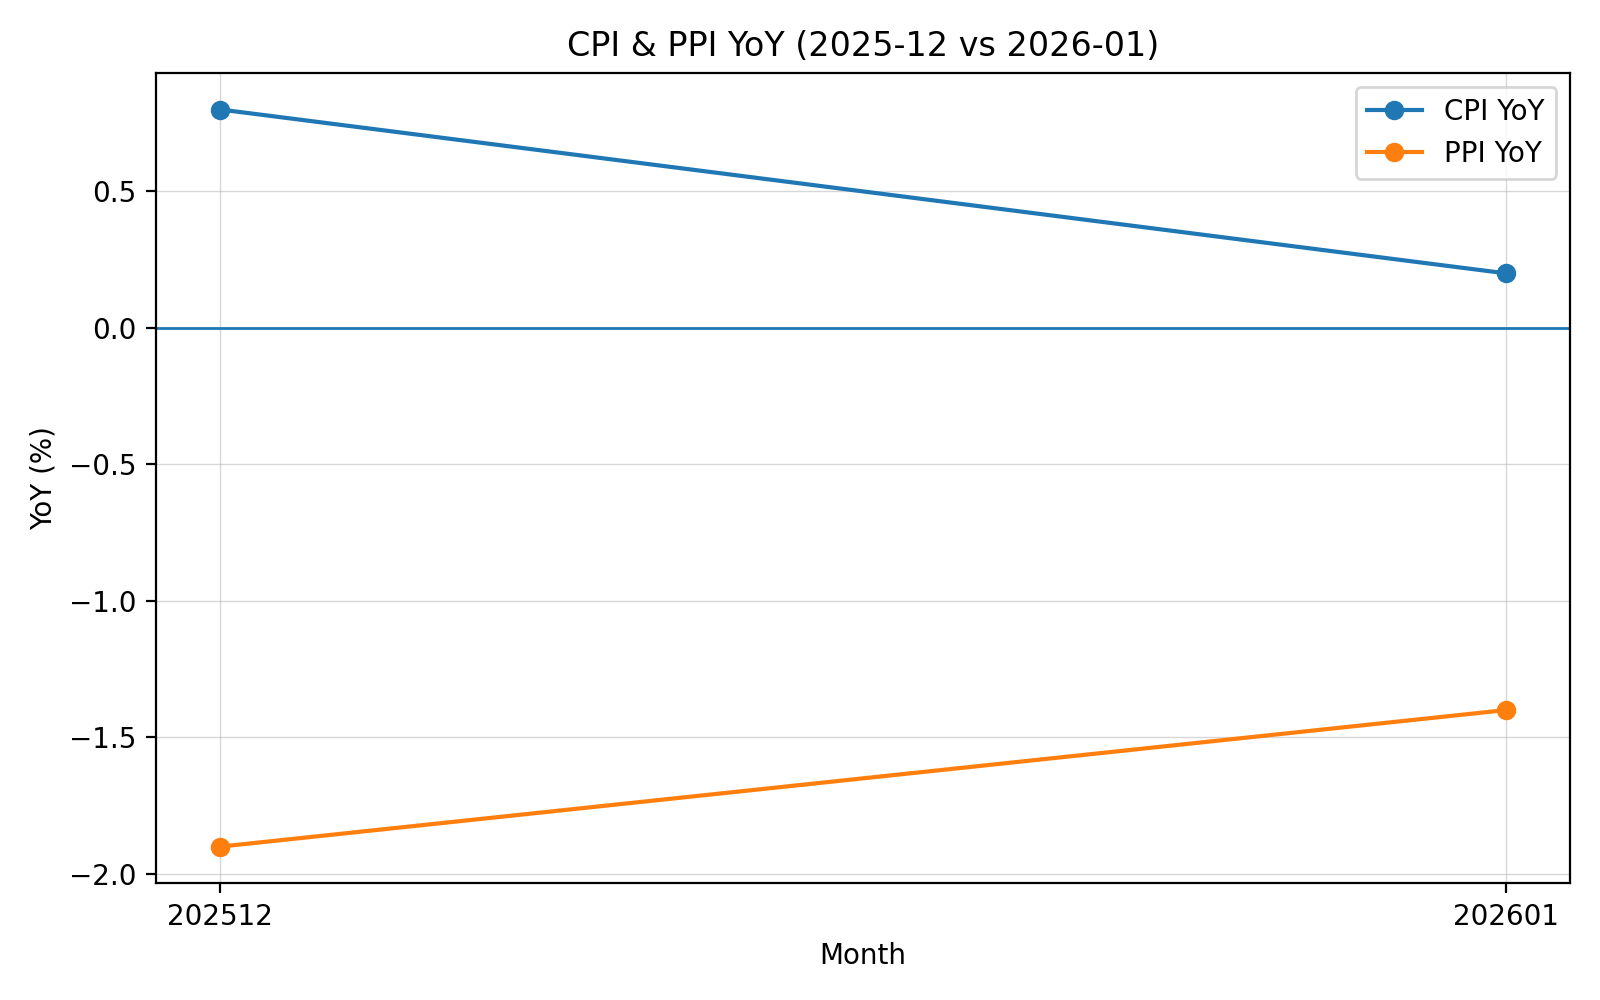
\includegraphics[width=0.80\textwidth]{figures/cpi_ppi_last2.png}
\caption{CPI \& PPI YoY（2025-12 vs 2026-01）}
\end{figure}

2025年12月CPI同比约0.8\%，
PPI同比约-1.9\%；
2026年1月CPI回落至0.2\%，
PPI回升至-1.4\%，
但仍处负值区间。
通胀水平整体偏低，
价格环境对长端利率形成一定约束。

% =========================
\section{政策与信用供给：MLF净投放与社融增量}
% =========================

\begin{figure}[H]
\centering
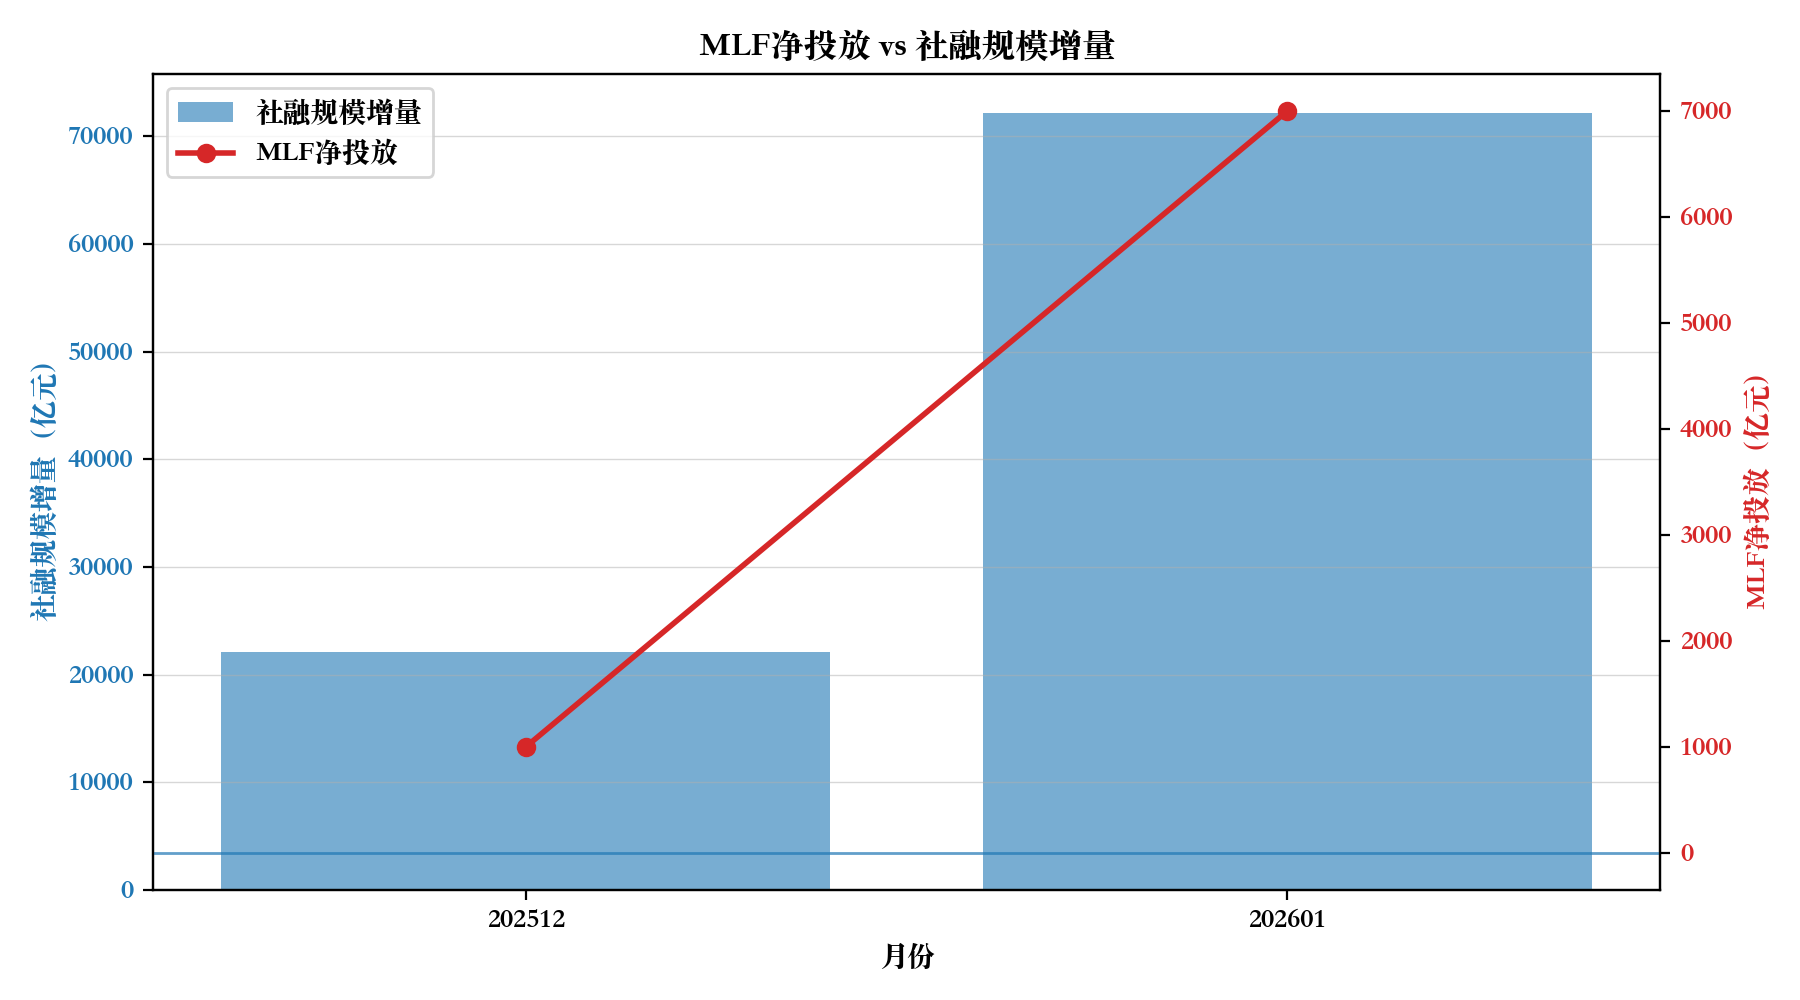
\includegraphics[width=0.92\textwidth]{figures/mlf_net_vs_social_total.png}
\caption{MLF净投放 vs 社融规模增量}
\end{figure}

2025年12月MLF净投放约1000亿元，
社融规模约2万亿元；
2026年1月MLF净投放升至7000亿元以上，
社融规模增至约7万亿元。
二者同步扩大，
显示政策层面对信用供给形成配合，
后续效果仍需观察实体景气的反馈。

% =========================
\section{综合判断与观察清单}
% =========================

\subsection{当前组合信号}
\begin{itemize}
  \item 资金面：跨年扰动后回归平稳（关注DR007中枢是否抬升）。
  \item 负债端：NCD利差用于监测银行负债压力是否“由短端向中期传导”。
  \item 曲线：期限利差走陡/走平需结合资金与供给共同解释。
  \item 宏观：社融扩张需验证其质量，PMI与CPI/PPI目前仍偏弱。
\end{itemize}

\subsection{未来两周/两月的关键观察指标}
\begin{enumerate}
  \item DR007是否持续高于政策利率附近的舒适区（观察是否趋势性偏紧）。
  \item NCD 3M/1Y是否跟随上行（判断负债压力是否“中期化”）。
  \item 10Y与DR007是否重新耦合：若资金偏紧 + 长端上行，则风险更大。
  \item 社融结构：票据与短贷占比 vs 中长贷/企业债占比变化。
  \item PMI是否回到50上方；PPI是否继续修复向0逼近。
\end{enumerate}

\section*{风险提示}
\begin{itemize}
  \item 财政供给超预期导致长端阶段性承压；
  \item 信用修复显著改善带动经济与通胀抬升；
  \item 海外利率上行或外部风险事件引发风险偏好切换。
\end{itemize}

\end{document}